    \subsection*{A benefit of clustering}
    
        One advantage for downstream applications is, there might be patterns that are more obvious if you only look at related segment of the data. For example:
        
        \begin{figure}[h]
            \centering
            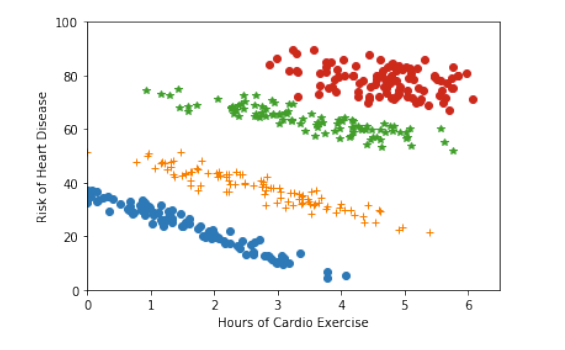
\includegraphics[width=0.65\textwidth]{images/clustering_images/simpsons_problem.png}
        \end{figure}
        
        If we take the data as a whole (\textbf{no} clustering), we would draw a \textbf{positive} regression: it seems that exercise and heart disease increase \textbf{together}. That doesn't make sense!
        
        But, if we divide it into \textbf{clusters}, based on age, we see a \textbf{negative} relationship: each individual group experiences \textbf{benefits} from exercise.
        
        This particular issue is called \textbf{Simpson's Paradox}.\\
        
        \begin{definition}
            \vocab{Simpson's Paradox} is when a \purp{trend} that appears in groups of data either \gren{vanishes} or \gren{reverses} when we look at all the data \purp{together}.
            
            It shows that sometimes, \purp{patterns} that we see may reflect how we're \gren{looking} at the data.
        \end{definition}
        
        Rest assured, you don't need to know this paradox by \textbf{name}! But it's important to \textbf{understand} possible problems like it: it'll make you more \textbf{responsible} in the future!